\documentclass[handout]{beamer}
\usepackage{graphicx}

\title{Using Language Models for Mathematics}
\author{Zhangir Azerbayev}
\institute{Yale University}
\date{2023}

\begin{document}

\frame{\titlepage}

\begin{frame}
\frametitle{Introduction}
How can we design a computer program that does mathematics better than any human?
\begin{itemize}
    \item Solve open problems
    \item Pose conjectures and create theories
    \item Convince mathematical community its proofs are correct\\~\
\end{itemize}
\pause
Questions I won't be talking about
\begin{itemize}
    \item How can we build tools for mathematicians?
    \item Does it matter whether we understand mathematics done by a machine?
\end{itemize}
\end{frame}

\begin{frame}
\frametitle{Approach 1: ask GPT}
The most obvious thing to try is to ask the language model to do math. How well does this work?\\~\ \pause

Minerva (Lewkowycz et al. 2022): 540B parameter transformer trained on 39B tokens of math. Based on PaLM, a general domain language model.
\begin{center}
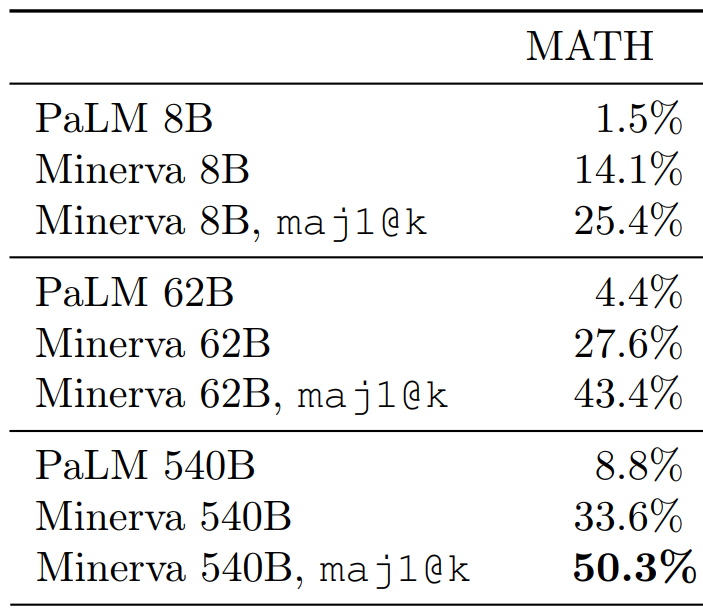
\includegraphics[width=0.5\textwidth]{img/minerva.png}
\end{center}
{\it MATH: a benchmark of high school and olympiad math problems}
\end{frame}

\begin{frame}
\frametitle{Approach 1: ask GPT}
{\bf GPT-4:}
\begin{center}
    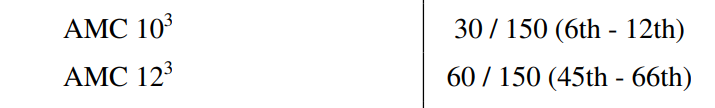
\includegraphics[width=0.75\textwidth]{img/gpt4.png} 
\end{center}
\end{frame}


\begin{frame}
\frametitle{Approach 1: ask GPT}
\begin{center}
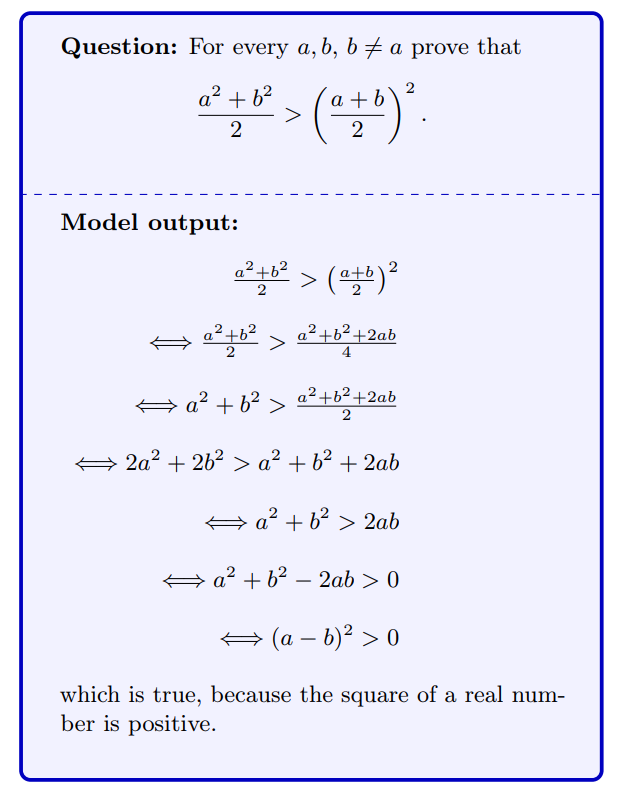
\includegraphics[width=0.45\textwidth]{img/minerva_example.png} 
\end{center}
\end{frame}

\begin{frame}
\frametitle{Background: scaling laws}
What happens when we keep feeding in more parameters and more data?\\~\

Loss function: $L(f) = -\sum_{x\in X}\log P(x | \theta)$\\~\

We're approximating the data distribution with $\mathcal{F}$, the set of $N$-parameter transformers. Let $f^*$ be the Bayes optimal classifier and $f_{\mathcal{F}} = \mathrm{argmin}_{f\in \mathcal{F}} L(f)$
\end{frame}

\begin{frame}
\frametitle{Background: scaling laws}
\begin{center}
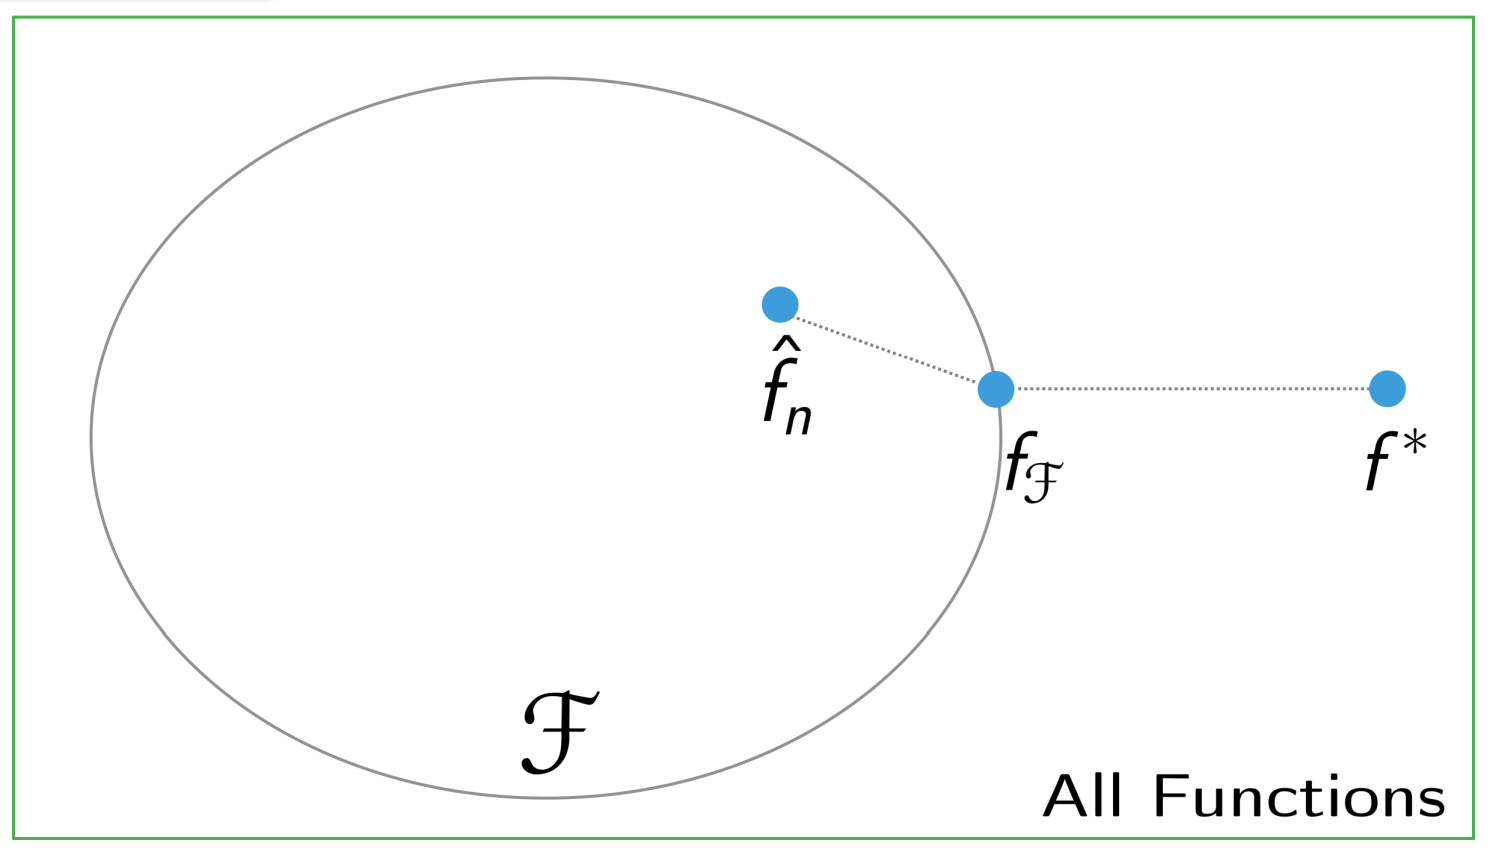
\includegraphics[width=0.45\textwidth]{img/excess_risk.png}
\end{center}
\begin{align*}
    \text{Excess risk}(\hat{f}) &= \underbrace{\left(L(f^*) - L(f_{\mathcal{F}})\right)}_{\text{approximation error}} + \underbrace{\left(L(f_{\mathcal{F}}) - L( \hat{f})\right)}_{\text{estimation error}}\\ 
                                &= \frac{A}{N^\alpha} + \frac{B}{D^\beta}
\end{align*}
\end{frame}

\begin{frame}
\frametitle{Background: scaling laws}
Hoffmann et al. 2022 (Chinchilla): most up to date empirical work on scaling laws. 
\begin{center}
    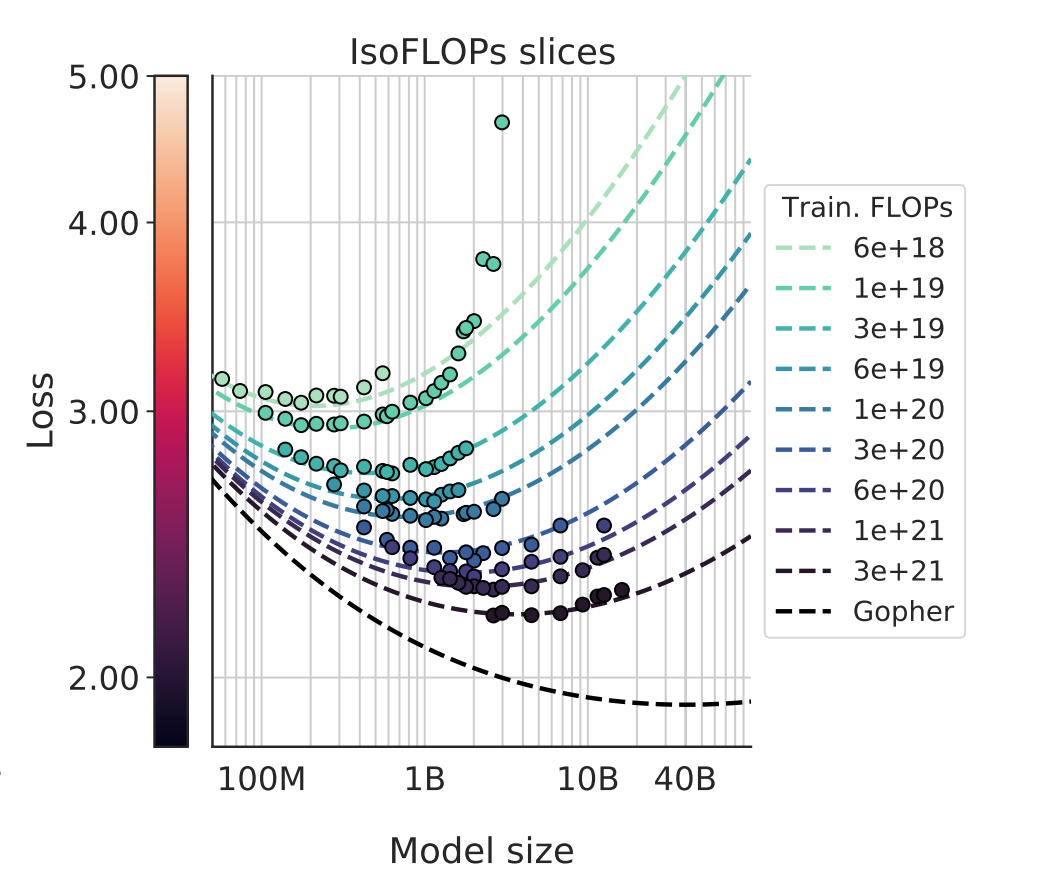
\includegraphics[width=0.45\textwidth]{img/chinchilla.png} 
\end{center}
$$L(\hat{f}) = 1.69 + \frac{406.4}{N^{0.34}} + \frac{410.7}{D^{0.28}}$$
\end{frame}

\begin{frame}
\frametitle{Approach 1: ask GPT}
Our model gets arbitrarily good with more parameters and more data.\\~\

So let's just ask our model to do mathematics in natural language. \\~\

\pause
We might be concerned about mistakes, but soon we will train a bigger model with a lower loss and we can ask that model to check the proof. Eventually, all errors will be caught because the loss of our models approaches the entropy of the text.
\end{frame}

\begin{frame}
\frametitle{Data limitations}
High quality mathematical text is extremely scarce. There is perhaps only $\sim 100$ billion tokens of it. This is tiny by language modelling standards.\\~\

As we increase the size of our dataset, the proportion of high-quality mathematics in it will vanish.\\~\

If we have infinite general domain data but finite mathematics data, can we still approach the entropy of the text?
\end{frame}

\begin{frame}
\frametitle{Scaling laws for transfer}
Suppose we have data from a distribution $P_1(\cdot)$, but we wish to model $P_2(\cdot)$. Then the best we can do is 
\begin{align*}
    \text{Excess risk}_2(\hat{f}) = &\left(L_2(g^*) - L_1(f^*)\right) - \left(L_1(f^*)-L_1(f_{\mathcal{F}}\right) + \\ & \left(L_1(f_{\mathcal{F}}) - L_1(\hat{f})\right)
\end{align*}
\pause
Thus for zero-shot transfer, the scaling law get is 
$$L_2(N, D_1) = \underbrace{S}_{\text{entropy}} + \underbrace{P}_{\text{penalty}} + \frac{A}{N^\alpha} + \frac{B}{D_1^\beta}$$
\end{frame}

\begin{frame}
\frametitle{Scaling laws for transfer}
In practice, we have a little bit of data $D_2$ from the target distribution (mathematics) that we can fine-tune on. \\~\

The penalty is some non-zero constant when $D_2=0$ and vanishes as $D_2\to\infty$. So it seems reasonable to posit that our scaling law is 

$$L_2(N, D_1, D_2) = S + \frac{A}{N^\alpha} + \frac{B}{D_1^\beta} + \frac{C}{D_2^\gamma}$$
\end{frame}

\begin{frame}
\frametitle{Empirical scaling laws for transfer}
Experiments with Pythia-1.4b model and math fine-tuning dataset (arXiv, stack exchange, formal math, numerical computing, etc.)
\begin{center}
    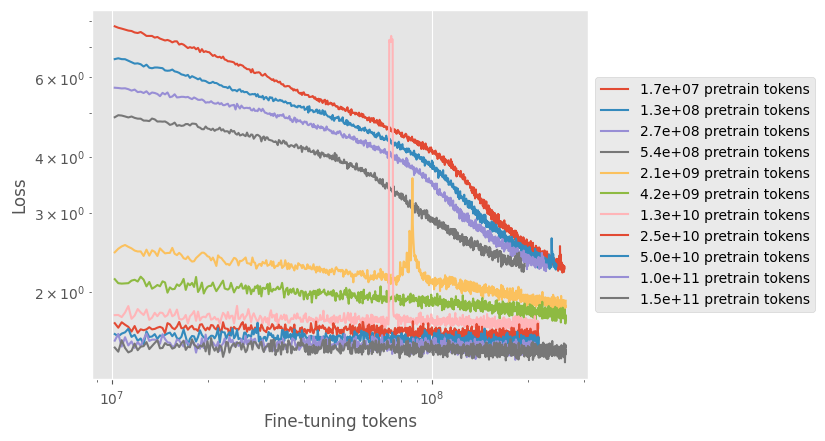
\includegraphics[width=1\textwidth]{img/ex1.png}
\end{center}
\end{frame}
\begin{frame}
\frametitle{Empirical scaling laws for transfer}
\begin{center}
    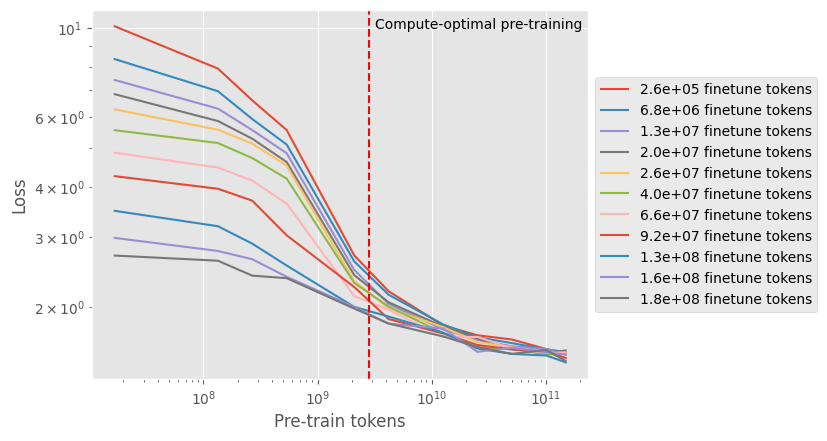
\includegraphics[width=1\textwidth]{img/ex2.png}
\end{center}
\end{frame}

\begin{frame}
\frametitle{Discussion}
It appears that there are limits to how much we can reduce loss on arXiv {\it with the data we have available to us}.\\~\

Although this analysis is not conclusive. We haven't tried varying model parameters yet (maybe there is an interaction term between $N$ and $D_2$), and we haven't varied data over enough orders of magnitude.\\~\

Our only option is to have the model generate its own data, i.e {\it reinforcement learning}
\end{frame}

\begin{frame}
\frametitle{Interactive Theorem Proving}
Interactive theorem provers are the ideal reinforcement learning ``environment'' for mathematics. \\~\

Proof checker catches incorrect reasoning and can be used to implement the reward model.\\~\

{\it pySagredo}: a basic tool for using language models to prove theorems in Lean 4.
\end{frame}

\begin{frame}
\frametitle{pySagredo}
PySagredo is a probabilistic program that samples from language model primitives. \\~\

Suppose you have some Lean code $T_0$ that is missing a proof. First, we sample a natural language proof sketch $S\sim P(S|T_0)$. The interactive theorem prover is able to deterministically give us its state: $L_n = f(T_n)$. \\~\

Proving proceeds by iteratively applying a probabilistic kernel $P(T_{n+1} | T_{n}, L_n, S)$. The kernel either corrects an error message (if there are any raised by $L_n$) or adds a new tactic step to the proof. When $L_n$ shows no goals or errors, the proof is finished.
\end{frame}

\begin{frame}
\frametitle{Probabilistic kernel: prompt}
\begin{center}
    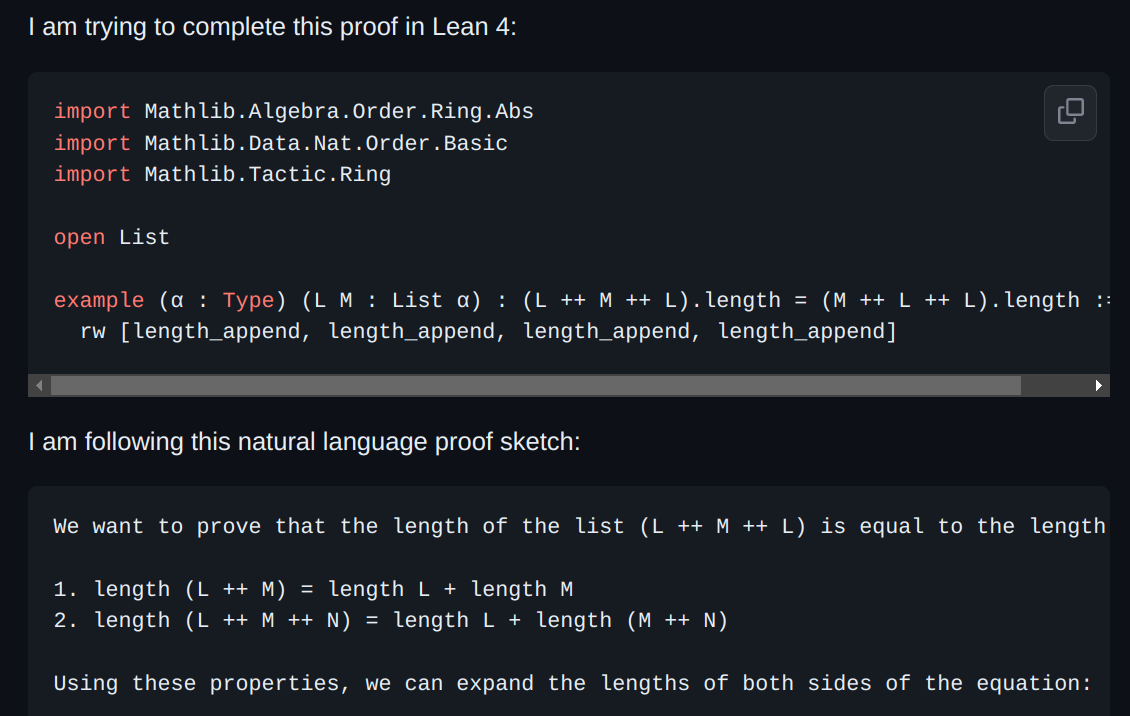
\includegraphics[width=1\textwidth]{img/s1.png}
\end{center}
\end{frame}
\begin{frame}
\frametitle{Probabilistic kernel: prompt}
\begin{center}
    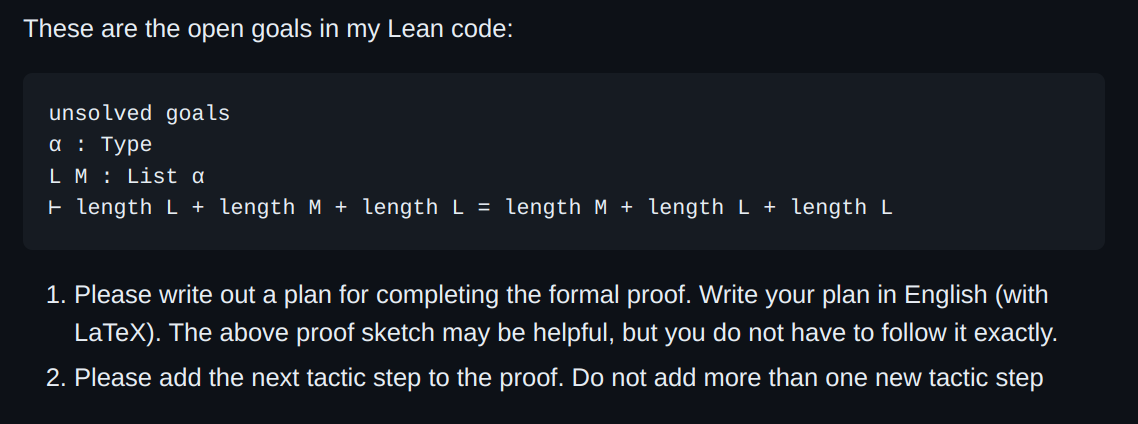
\includegraphics[width=1\textwidth]{img/s2.png}
\end{center}
\end{frame}
\begin{frame}
\frametitle{Probabilistic kernel: response}
\begin{center}
    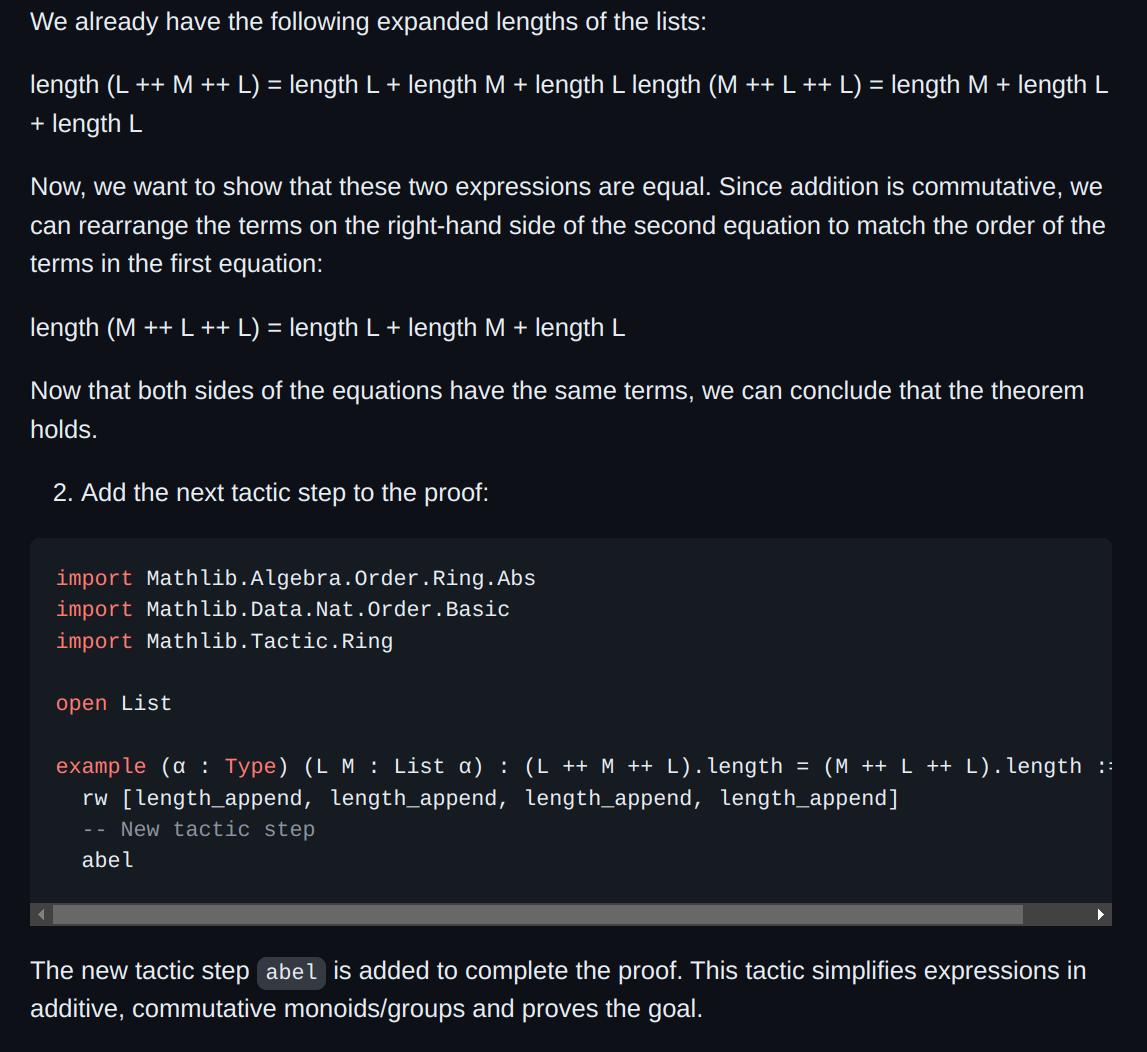
\includegraphics[width=0.75\textwidth]{img/s3.png}
\end{center}
\end{frame}

\begin{frame}
\frametitle{Closing the loop}
We've seen language models can 
\begin{itemize}
    \item Learn mathematics, to some modest level, from behavior cloning.
    \item Interact with an ITP environment.\\~\
\end{itemize}
\pause
Can we design an algorithm that allows language models to {\it learn from their interaction with the ITP environment}.\\~\

\pause
Prior efforts to use reinforcement learning for language and reasoning don't inspire optimism:\\~\
\begin{itemize}
    \item Tree search + expert iteration saturates quickly. Algorithm doesn't cope with complex action spaces well. 
    \item RL from Human Feedback doesn't help much with capabilities.
\end{itemize}
\end{frame}

\begin{frame}
\frametitle{Closing the loop}
RL consists of two steps
\begin{enumerate}
    \item Try new things (exploration)
    \item Keep doing the things that gave high reward. (exploitation)\\~\
\end{enumerate}
We don't have any ideas for (1) except ``do something random''. \\~\

\pause
Maybe productive exploration is an emergent property of a sufficiently good supervised policy?
\end{frame}




\end{document}
